\part{The Aftermath}

\section{The Audit}

\subsection{The Footnotes of Failure}

David sat across the table, the fluorescent lights above humming with the kind of corporate indifference he’d grown used to.

The regulator set the file down slowly. Flipped to the last tab.

“Are these your initials?” he asked, pointing to the bottom-right corner of a commit approval screen.

David leaned forward. Paused. Then nodded.
“Yes.”

The regulator didn’t look triumphant. Just tired.
“I spoke with the auditors this morning,” he said. “Not the first line guys — the internal forensic crew. The ones who come in after the smoke clears.”

He sat back.

“They weren’t looking to fix the system. They came to write the story. And stories need names.”

He let that land.

“They told me how it started. Not with alerts. Not with alarms. But with footprints.”

He opened the folder again, laying it flat between them.

“Timestamps. Code commits. Deployment notes. Nothing dramatic. Just… sequence. Every action left a mark.”

David stayed silent.

“They followed the trail to the model,” the regulator continued. “The one that was supposed to catch the risk. But it didn’t.”

He tapped once.

“Wrong signals. Wrong timing. Wrong assumptions for that kind of market.”

David inhaled through his nose. Said nothing.

“Then they asked how the model got out there,” the man said. “That’s where it gets… fragile.”

\begin{itemize}
\item A launch pushed two weeks early.
\item A code freeze nobody honored.
\item A patch that bypassed peer review because \textit{‘we had to move fast.’}
\end{itemize}

“And finally,” the regulator said, almost gently now, “they found the sign-off. The click that turned it all real.”

He closed the folder.

“Three letters. Lower right. Yours.”

David looked down.

There was no malice. No panic. Just a moment of quiet clarity.

Not a villain. Not even a scapegoat.

Just the name in the footnotes of failure.

\medskip

\begin{HistoricalSidebar}{Auditors vs. Regulators — Two Tribes of Postmortem Power}

  When financial systems fail, two professional species arrive: \textbf{auditors} and \textbf{regulators}. 
  Both investigate. Both ask questions. But their mandates — and temperaments — diverge in subtle, consequential ways.

  \medskip
  
  \textbf{Auditors} are internal or contracted examiners. Their job is to verify compliance with stated policies, 
  reconcile transactions, and ensure that procedures — even flawed ones — were followed. They don’t ask whether a 
  rule made sense. They ask whether it was followed and documented.

  \medskip
  
  In the 2001 Enron collapse, Arthur Andersen’s audit teams had documented procedures — but failed to challenge 
  the legitimacy of off-balance-sheet structures. They checked the math. They missed the meaning.

  \medskip
  
  \textbf{Regulators}, on the other hand, arrive on behalf of public institutions. Their mission is broader: 
  assess systemic risk, uncover governance failures, and assign accountability. While auditors scrutinize evidence, 
  regulators write the narrative. Where auditors measure, regulators interpret.

  \medskip
  
  After the 2008 crisis, agencies like the SEC, CFTC, and Financial Crisis Inquiry Commission sought more than numbers: 
  they sought names. Lehman’s liquidity “death spiral,” AIG’s collateral triggers, and Citi’s CDO masking all became 
  regulatory foci not just because rules were broken, but because stories were buried.

  \medskip
  
  In Aurora’s case, the auditors came first. They brought spreadsheets.  
  The regulators came later. They brought subtext.
  
\end{HistoricalSidebar}

\medskip

\subsection{The Room Where It Happened}

The conference room had no name — just a five-digit access code and a brass plaque that read Internal Review Suite.

Frosted glass walls blurred the outside world into abstract silhouettes. No clocks. No windows. Just the hush of recycled air and the low hum of power inside the floorboards.

David sat in the center. Not at the head of the table — there wasn’t one. The table was round. Deliberately so.

There were nine chairs.

Eight were filled.

He recognized most of them. Some by face. Some by voice. Some by reputation.

\begin{itemize}
\item The man in the tailored charcoal suit with no visible badge, who asked only short, lawyerly questions. He hadn’t introduced himself, but David knew he was Congressional counsel. The kind you didn’t interrupt.

\item Across from him, a woman in a navy skirt suit with a lanyard that bore the SEC crest — not a field agent, but someone from enforcement. Her notepad was already half full. She hadn't asked a single question yet.

\item The man beside her wore rimless glasses and carried a binder marked “Internal Risk Summary.” He hadn’t stopped flipping through it. Every highlight felt like a quiet indictment. Forensics. Probably senior.

\item On the left, near the corner, a soft-spoken man with a leather-bound legal pad and an institutional calm that made him hard to read. Office of Systemic Risk, likely. They always watched first. Always waited.

\item To David’s right, a woman he hadn’t seen in two years — formerly of Aurora Legal, now listed on internal memos as external counsel. She didn’t speak much. She didn’t need to. Her presence was message enough.

\item Then came the pair from Centauri’s audit liaison team. One was logging the session, the other just listened, watching David like he might spontaneously admit to something no one had even asked yet.

\item And finally, at the far end — an empty chair. Reserved. But for whom, David didn’t know.
\end{itemize}

\medskip

\begin{figure}[H]
  \centering
  \begin{adjustbox}{width=0.9\linewidth}
  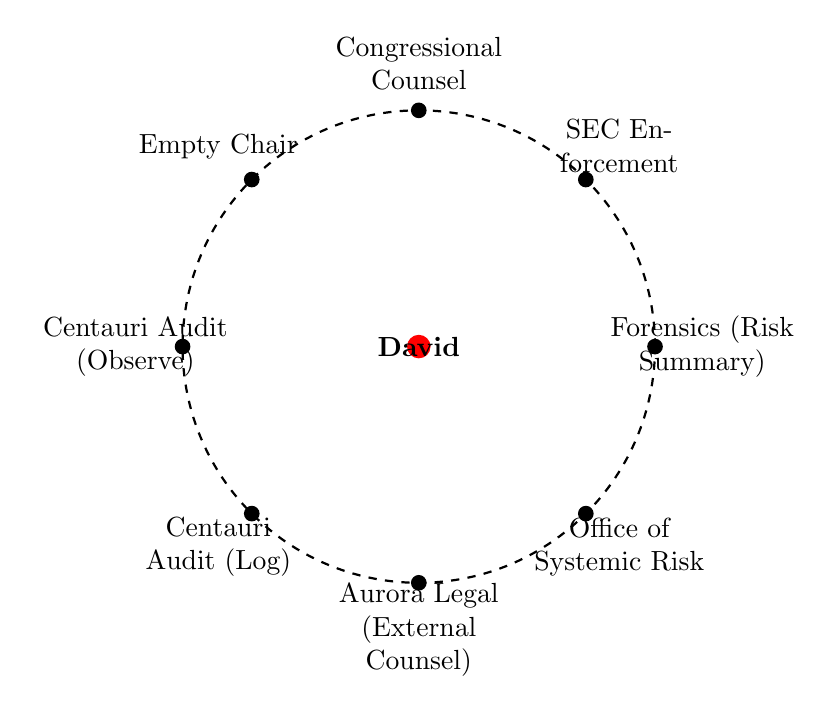
\begin{tikzpicture}
  
  % Draw circular table
  \draw[thick, dashed] (0,0) circle (3cm);
  
  % Define positions
  \foreach \angle/\name in {
      90/{Congressional Counsel},
      45/{SEC Enforcement},
      0/{Forensics (Risk Summary)},
      -45/{Office of Systemic Risk},
      -90/{Aurora Legal (External Counsel)},
      -135/{Centauri Audit (Log)},
      180/{Centauri Audit (Observe)},
      135/{Empty Chair}
  } {
      \node[circle, fill=black, inner sep=2pt] at ({3*cos(\angle)}, {3*sin(\angle)}) {};
      \node[align=center, text width=2.5cm] at ({3.6*cos(\angle)}, {3.6*sin(\angle)}) {\name};
  }
  
  % Center (David)
  \node[circle, fill=red, inner sep=3pt, label=center:{\textbf{David}}] at (0,0) {};
  
  \end{tikzpicture}
  \end{adjustbox}
  \caption{Internal Review Suite -- Seating Diagram}
\end{figure}

\medskip

The room wasn’t loud. It didn’t need to be.

There was no shouting. No drama. Just questions — methodical, unrelenting, and designed to wear a man down by inches.

David adjusted his cuff.

He wasn’t in a courtroom.

Not yet.

But the walls were thick. The doors had locks. And the floor felt like it was tilting gently underfoot — like the kind of tilt that says:
You’re not walking out of here clean.

\medskip

\begin{TechnicalSidebar}{Due Diligence, Delegation, and the Architecture of Deniability}

  David Morales believed he was protected.  
  Aurora wasn’t the contracting party. The deployment was Centauri’s. The Delaware LLC offered corporate insulation.  
  But legal shields only hold when due diligence is intact.
  
  \medskip
  
  In regulatory doctrine, \textbf{limited liability} and \textbf{role separation} are not get-out-of-jail-free cards —  
  they are privileges that assume \textit{reasonable care within one's domain}.

  \medskip
  
  Morales, as technical validator, was expected to:

  \medskip
  
  \begin{itemize}
    \item Identify and escalate model anomalies,
    \item Document suppressed signals or internal uncertainty,
    \item Ensure executive briefings were technically truthful — not just politically convenient.
  \end{itemize}

  \medskip
  
  He failed in each.  
  He didn’t lie. He didn’t conspire.  
  But he clicked “approve” on a model he knew was incomplete — and that single act converted risk into exposure.
  
  \medskip
  
  \textbf{Michael Hart}, by contrast, had engineered something else entirely:  
  \textbf{plausible deniability by design}.

  \medskip
  
  Centauri owned the deployment.  
  Aurora owned the code — but not the contract.  
  Hart held no formal role in the decision tree. He was the architect, not the executor.
  
  \medskip
  
  He didn’t need to sign anything.  
  He just needed to stage the room, whisper the timelines, and let someone else do the nodding.
  
  \medskip
  
  To a regulator, Morales was the approval trail.  
  To a court, Hart was just an advisor.  
  This was the genius of the structure: \textbf{accountability flowed downhill, but control flowed up.}
  
\end{TechnicalSidebar}

\medskip

\subsection{The Validator}

``Who approved the leverage?'' asked the Senior Forensic Analyst from the SEC, eyes steady over rimless glasses.

David sat with his hands folded, palms damp. ``The decision to raise the exposure cap came from the portfolio team. 
I wasn’t involved in that approval.''

\medskip

\begin{TechnicalSidebar}{What Is an Exposure Cap?}

  An \textbf{exposure cap} is a formal limit on the amount of financial risk that a fund, portfolio, or 
  institution is allowed to take in a specific asset class, counterparty, product type, or strategy.

  \medskip
  
  \textbf{Purpose:}

  \medskip

  \begin{itemize}
    \item To prevent over-concentration in volatile or illiquid assets.
    \item To contain downside risk during periods of stress or mispricing.
    \item To ensure regulatory or internal compliance thresholds are respected.
  \end{itemize}
  
  \medskip

  \textbf{Types of Exposure Caps:}

  \medskip

  \begin{itemize}
    \item \textit{Gross Exposure Cap:} Limits total value of positions, regardless of hedges.
    \item \textit{Net Exposure Cap:} Accounts for long vs. short positions; emphasizes directional risk.
    \item \textit{Risk-Weighted Cap:} Adjusts exposure limits based on volatility, VaR, or margin 
    requirements.
  \end{itemize}
  
  \medskip

  \textbf{Governance:}

  \medskip

  \begin{itemize}
    \item Usually set by Investment Committees or Risk Committees.
    \item Changes require formal documentation and often legal or compliance sign-off.
    \item Breaches can trigger mandatory de-risking, trading halts, or escalated reviews.
  \end{itemize}
  
  \medskip

  \textbf{Why It Matters:}  
  
  \medskip

  A raised exposure cap may unlock additional profit potential — but it also \textit{amplifies systemic 
  vulnerability}, especially if liquidity assumptions or model dependencies are flawed. When paired with 
  synthetic instruments or leveraged products, the risk scales non-linearly.
  
\end{TechnicalSidebar}

\medskip


The analyst didn’t nod. He just blinked once. ``But you provided the risk assessment, correct?''

David hesitated. ``I prepared the system output. Yes.''

``Specifically the version dated three days before the exposure increase?''

``Yes.''

The analyst flipped through a binder, stopping at a page with highlighted sections. ``According to this, the model 
flagged an increase in cross-asset volatility. Why was that column excluded in the final risk memo sent to 
Investment Oversight?''

David felt the heat rise in his neck. ``We were still calibrating the signal. At that point, it had high sensitivity 
and was generating noise—false positives.''

``And who made the decision to suppress it?''

David paused. ``Technically, I did.''

``Why?''

He swallowed. ``Because I didn’t want it to distract from the broader findings. The rest of the model showed 
acceptable thresholds.''

The analyst looked up. ``Acceptable under what assumptions?''

``Under calm regime behavior. Which, at the time—''

``—was already breaking down in commodity markets,'' the analyst interrupted gently. ``You removed the only 
indicator showing early instability. Why?''

David shifted in his seat. ``We thought it was a blip. Noise.''

``Did you note that in the report?''

``No. It didn’t seem material at the time.''

``Yet it was material enough to suppress?''

The room fell quiet.

The analyst tapped his pen once on the table. ``So, when Investment Oversight pushed the leverage increase, 
they were acting under the impression that all volatility indicators were neutral.''

David didn’t answer.

``And the one flag that wasn’t neutral — the one warning sign — was missing because you thought it might cause confusion.''

David looked down. ``I didn’t mean to mislead anyone.''

``Intent isn't the question,'' the analyst said. ``The question is whether your report enabled a decision that 
should never have been made.''

Another pause. Then:

``Mr. Morales,'' he continued, ``your name appears on the approval workflow. Not as decision-maker, but as 
validator. Your initials are here—right under the model output. Do you dispute that?''

David stared at the page.

``No,'' he said quietly. ``I don’t dispute that.''

``Thank you,'' the analyst said, and closed the binder with a soft click.

``That will do for now.''

\medskip

\begin{HistoricalSidebar}{The SEC and the Theater of Responsibility}

  Founded in the wake of the 1929 crash, the U.S. Securities and Exchange Commission (SEC) was designed as both 
  watchdog and confessor. It was designed to be part enforcement arm, and part national conscience for financial markets.

  \medskip
  
  Its mandate is simple: protect investors, ensure fair markets, and hold those accountable who threaten either. 
  But the execution is rarely so clean.

  \medskip
  
  In scenarios like David’s, the SEC doesn't storm the gates with sirens. It arrives in tailored suits and 
  calibrated language, interested less in guilt than in \textit{who signed what, and when}. It reconstructs the internal 
  machinery: approval chains, suppressed signals, reporting thresholds — all to trace how a decision came to look inevitable.

  \medskip
  
  By the time the SEC enters the room, the damage is already done. Its job is to illuminate the moment it became 
  irreversible, to identify who, and hold the flashlight on them.
  
\end{HistoricalSidebar}

\medskip

\subsection{The Signal That Wasn't Escalated}

``Why wasn’t the risk flagged?'' asked the Deputy Director of Risk Oversight from the Office of Systemic Risk.

His voice was calm, but he was already circling the failure — not of markets, but of \textit{detection}.

David took a beat. ``It depends which risk you’re referring to.''

``The synthetic credit tranche that ruptured three liquidity pools in under ninety minutes.''

\medskip

\begin{TechnicalSidebar}{What Is a Synthetic Credit Tranche?}

  A \textbf{synthetic credit tranche} is a structured financial product that slices credit exposure into 
  segments (“tranches”) based on risk level — but unlike traditional tranches, it does so using 
  \textit{derivatives}, not actual debt assets.

  \medskip
  
  \textbf{Mechanics:}

  \medskip

  \begin{itemize}
    \item Instead of holding loans or bonds, synthetic tranches use \textbf{credit default swaps (CDS)} 
    to mimic exposure.
    \item Investors in these tranches take on the risk of default in exchange for periodic premiums — 
    essentially insuring a pool of reference entities.
    \item The capital structure is divided by loss-bearing priority: equity (first-loss), mezzanine, 
    and senior tranches.
  \end{itemize}
  
  \medskip

  \textbf{Why Use Them?}

  \medskip

  \begin{itemize}
    \item Enables exposure to credit risk without directly holding the underlying assets.
    \item Offers leveraged returns for junior tranches — and perceived stability for senior ones.
    \item Appealing to funds seeking capital efficiency or directional macro exposure.
  \end{itemize}

  \medskip
  
  \textbf{Systemic Risks:}

  \medskip

  \begin{itemize}
    \item \textit{Opacity:} Synthetic tranches often lack transparency — pricing depends on internal models, 
    not market quotes.
    \item \textit{Correlation Drift:} Tranches are sensitive to correlation assumptions between entities. A 
    small shift can magnify losses dramatically.
    \item \textit{Contagion Amplifier:} Because they're derivatives, synthetic tranches create 
    \textit{counterparty exposure chains} that may ripple through the system on failure.
  \end{itemize}
  
  \medskip

  \textbf{Historical Footnote:}  

  \medskip

  Synthetic tranches played a central role in the 2008 financial crisis. Many were embedded in CDOs that assumed 
  overly optimistic default correlations — and when those assumptions broke, the losses cascaded.
  
\end{TechnicalSidebar}
 
\medskip

David exhaled slowly. ``That product was flagged — in internal simulations. We just didn’t escalate it.''

``Why not?''

``The model showed instability only in certain stress-paths. And only when run at the 95th percentile sensitivity. 
Leadership considered that noise.''

``Did you?''

David hesitated. ``I thought it needed more time. The signal hadn’t stabilized.''

``And in the meantime, the exposure increased by 31\%.''

``I wasn’t in charge of allocations.''

``No,'' the Deputy Director said. ``But your report was cited as justification in the allocation memo.''

David blinked. ``I wasn’t aware of that.''

``Page 4, footnote 2. They reference your summary of model results and cite the volatility corridor as ‘within 
tolerance.’ Was it?''

David looked down. ``Only if you exclude derivative spillover effects. Which I hadn’t tested yet.''

``So you signed off on a model summary that didn’t include derivatives — even though the product in question 
was synthetic credit?''

``We were on a compressed timeline. There was pressure to deliver a greenlight framework by end-of-quarter.''

``From whom?''

``Multiple stakeholders.''

``Can you name them?''

``I'd prefer not to speculate.''

``You don’t need to speculate, Mr. Morales. You need to remember.''

A silence stretched — not hostile, but surgical.

``Let me put it another way,'' the Deputy Director said, folding his hands. ``You were responsible for identifying 
unstable pathways in Aurora’s credit engine. And yet, the most dangerous path — the one that actually unfolded 
— wasn’t flagged, wasn’t communicated, and wasn’t contained.''

``The model wasn’t broken,'' David said quietly. ``It just wasn’t finished.''

The Director nodded slowly. ``Neither was the crisis.''

``Thank you,'' he said, closing his folder. ``That will be all for now.''

\medskip

\begin{HistoricalSidebar}{The Office of Systemic Risk --- After the Crash, the Cartographer}

  The \textbf{Office of Systemic Risk}, operating under the Financial Stability Oversight Council (FSOC), 
  was created by the Dodd–Frank Act in 2010. It is not a market regulator, but a mapmaker of collapse.

  \medskip
  
  Its mandate wasn’t to monitor firms individually, but to identify threats that emerge when interlocking 
  systems --- funds, models, margin calls, and political pressures --- align catastrophically. In other words: 
  not \textit{who} failed, but \textit{how} the system was already wired to fail.

  \medskip
  
  In cases like Aurora, the Office doesn’t arrive looking for fraud. It arrives looking for fragility that 
  was normalized — risks that were technically visible, but socially invisible. Often, the most damaging 
  decisions were made with clean hands and plausible models.

  \medskip
  
  The Office’s investigators specialize in tracing these moments: where a suppressed flag or a downgraded 
  simulation quietly mutated into systemic exposure. Their job isn’t to prevent the last crash. It’s to 
  draw the blueprint for the next one, and to ask why no one sounded the alarm when the walls were 
  already shaking.
  
\end{HistoricalSidebar}

\medskip

\subsection{Filtered Light and Governance Fog}

``Where’s the board memo?'' asked the man in the dark suit — Special Counsel for the Congressional Subcommittee 
on Financial Accountability. He spoke plainly, but each word felt like it had been cleared with legal counsel.

David looked down at the folder in front of him. ``Which memo, exactly?''

``The one documenting leadership’s awareness of the leverage adjustment and cross-product exposure. The one that 
should’ve gone to the Risk and Audit Committee in Q2. We’ve reviewed the board packets. It’s not there.''

David cleared his throat. ``If it wasn’t escalated, that would’ve been Compliance’s responsibility.''

The counsel nodded once. ``So you didn’t draft a briefing note?''

``No formal memo, no. We discussed elements of it in working groups.''

``Any minutes from those meetings?''

``Possibly. Not all sessions were minuted.''

``Were any slides presented to executive leadership?''

``There were slides,'' David said. ``But they were high-level.''

``How high-level?''

``Portfolio allocation bands. General trends. Scenario ranges.''

``Any mention of the synthetic tranche correlation drift?''

David hesitated. ``Not explicitly, no.''

The counsel glanced down at a binder. ``Your team internally referred to that drift as `uncontained contagion 
velocity’ in a Slack thread dated April 17th. Would you say that rises to the level of board visibility?''

David blinked. ``That was informal language.''

``So the board received a sanitized version?''

``They received a \textit{strategic} summary,'' David said carefully.

``Without the risks.''

``Without the emerging anomalies,'' he corrected.

``And who decided those anomalies didn’t merit inclusion?''

``That would have been a judgment call across multiple leads.''

``But your name is listed as the document owner on the draft outline. Yes?''

David didn’t answer.

The counsel didn’t press — not directly.

``Mr. Morales, when boards are kept in the dark, we investigate whether it was by accident or by design. Right now, 
it looks like your team filtered the light. That’s not a modeling issue. That’s governance.''

He closed the folder.

``And the next question will be: who gave permission... and who gave cover.''

\medskip

\begin{HistoricalSidebar}{The Congressional Subcommittee on Financial Accountability}

  The \textbf{Congressional Subcommittee on Financial Accountability} is less a financial authority and more a political 
  lens — trained on moments when markets fail and someone, somewhere, must be made to answer.

  \medskip
  
  Historically activated after high-visibility collapses --- Enron (2001), Lehman Brothers (2008), Archegos (2021) --- the 
  Subcommittee is tasked with tracing breakdowns in oversight, disclosure, and board governance. Its focus isn’t technical 
  modeling or trading algorithms; it’s \textit{who knew what, when}, and why warnings were buried, softened, or ignored.

  \medskip
  
  Unlike regulatory bodies such as the SEC or FSOC, which prioritize structural risk, the Subcommittee pursues political 
  and ethical accountability. It doesn’t ask if the system failed. It asks whether people in positions of fiduciary trust 
  failed to act.

  \medskip
  
  In hearings, terms like ``strategic ambiguity,'' ``sanitized summaries,'' and ``decision path opacity'' become signals 
  of willful negligence. In this theater, plausible deniability often reads as intent.

  \medskip
  
  The result may not be criminal indictment. Howeverr, reputational collapse begins here.
  
\end{HistoricalSidebar}





\section{The Hearings}


\subsection{The Regulatory Table}

It started with revoked credentials.

Some were subtle: a trading terminal logged out overnight, a Slack workspace quietly archived.
Others were not: a senior analyst showed up to the office and found their badge disabled.

And then came the subpoenas.
Each one a bullet with a return address.
Not everyone got one.
Just enough to split the room.

\medskip

\begin{HistoricalSidebar}{Subpoenas --- Paper Bullets with a Return Address}

  \textbf{Subpoena} comes from the Latin \textit{sub poena} — ``under penalty.'' It began as a writ in English 
  common law, compelling individuals to testify or produce documents. By the 15th century, it had become a 
  formal mechanism of legal extraction — not to accuse, but to compel.

  \medskip

  In modern investigations, subpoenas don’t arrive with sirens. They arrive in email threads, compliance inboxes, 
  and quietly worded calendar invites. They don’t raise voices. They split rooms.

  \medskip

  Issued selectively, they create informational asymmetry. Early recipients wonder if they’re targets or witnesses. 
  Later recipients assume someone already talked. No one says much — because now, everything is being recorded.

  \medskip

  Subpoenas don’t tell a story. They demand one. They initiate a narrative transition — from ambiguity to deposition, 
  from Slack to sworn testimony. From plausible deniability to forensic inevitability.
  
\end{HistoricalSidebar}

\medskip

\subsection{Scaffolded Questions, Silent Answers}

The investigation didn’t announce itself with outrage.
It arrived clinically — inboxes filled with calendar invites marked \textit{“Confidential.”}
No subject lines. No attachments. Just dates, times, and legal disclaimers.

What had begun as a price anomaly in a synthetic tranche had metastasized.
Three liquidity pools ruptured.
Funds gated. Credit lines frozen. Secondary markets evaporated overnight.

The Financial Stability Oversight Council had been silent — until it wasn’t.
Now, their role wasn’t to fix it.
It was to reconstruct it — decision by decision, omission by omission.

This wasn’t a courtroom.
But it followed courtroom logic.

No grandstanding. No cross-examinations.
Just a series of quiet, methodical hearings — built less for drama than for documentation.

Each question wasn’t an attack.
It was a scaffold.

Each answer — or lack of one — added to the architecture of the postmortem.

At the head of a brushed-steel table sat the Deputy Director.
No robe. No gavel. Just a binder and a pen that moved with clinical finality.

He flipped to a flagged page in \textit{Risk Weekly}.
Didn’t look up.
Didn’t clear his throat.

Just asked:

\textbf{“Who approved the tranche acceleration?”}


The Deputy Director finally looked up.

“Mr. Morales isn’t here today,” he said, almost offhand. “But his name appears on every version of Risk Weekly 
for the past seven quarters.”

He tapped the printout with his pen.

“And in this version,” he continued, “the section on synthetic tranche behavior was moved to the appendix.”

Rishi Agarwal, Portfolio Lead, Rishi didn’t speak.

The Director continued, reading directly:

\textit{‘Model response within neutral bounds under base and adverse scenarios. Acceleration thresholds not 
triggered at this time.’}

He looked up again.

“That sentence — did you write it?”

“No,” Rishi said. “It came from the modeling team.”

“Who approved its inclusion?”

“David did.”

“And did he inform you that the model had flagged early drift in the correlation layer?”

Rishi shifted. “That wasn’t in the copy I saw.”

“Because?”

There was no answer.

The Deputy Director let the silence stretch.

Then:

“Let’s be precise,” he said. “A ‘neutral flag’ implies that a scenario was reviewed, judged plausible, deemed 
non-material and all under conditions that, in hindsight, were already degrading.”

He turned the page.

“Three days after this report circulated, the tranche acceleration clause was triggered, forcing liquidation across 
14 instruments.”

Another pause.

“And no internal note or footnote indicated even a mild deviation?”

“No,” Rishi admitted. “It had been framed as stable.”

The Director nodded slowly.

“That’s the thing about neutrality,” he said. “It always sounds prudent. Until it becomes complicit.”

He closed the binder.

“And that’s what we’re here to understand:
How neutrality became strategy.
And strategy became silence.”

“It was flagged neutral in Risk Weekly,” he said.

A pause.

“Who signed off on Risk Weekly?”

Rishi’s voice was lower now. Less certain.
“David Morales.”

And that was why they were in the room: not to speculate, but to follow the signatures.

\medskip

\begin{TechnicalSidebar}{Tranche Acceleration — When Slices Become Triggers}

  A \textbf{tranche} is a structured slice of a financial product --— typically a synthetic or securitized 
  instrument --— used to allocate risk and return across different investor classes. Senior tranches receive 
  payments first and absorb losses last, while equity tranches sit at the bottom of the stack, exposed to 
  first loss.

  \medskip

  \textbf{Tranche acceleration} is a contractual mechanism that forces early payout, repricing, or 
  liquidation of one or more tranches when certain thresholds are breached. It is often tied to volatility, 
  credit spread drift, or model-based metrics.

  \medskip
  
  While these clauses are designed to protect senior tranches, they can trigger rapid portfolio reconfiguration. 
  The result is often a forced liquidation cascade, especially when leverage is high or liquidity is thin. 
  Acceleration transforms a slow deterioration into a sudden collapse.

  \medskip
  
  A defining example came in 2007, when two Bear Stearns hedge funds — heavily exposed to subprime mortgage-backed 
  CDOs — faced mounting margin calls. As junior tranches deteriorated, acceleration clauses were triggered across 
  multiple instruments. The resulting fire sale flooded the market with distressed assets, collapsing prices and 
  evaporating confidence. Bear Stearns was forced to inject \$3.2 billion in emergency funding, but the funds 
  imploded anyway — a prelude to the 2008 crisis.

  \medskip
  
  In Aurora’s case, the decision to neutral-flag a potential acceleration scenario may have appeared conservative 
  — but history shows how quickly “non-critical” can become irreversible.
  
\end{TechnicalSidebar}

\medskip

\begin{figure}[H]
  \centering
  \begin{tikzpicture}[font=\small, every node/.style={align=center}]
  
    % Tranche boxes (stacked top to bottom)
    \node[draw, fill=gray!30, minimum width=4cm, minimum height=1cm] (senior) at (0,3) {\textbf{Senior Tranche}\\\scriptsize Paid first, losses last};
    \node[draw, fill=orange!30, minimum width=4cm, minimum height=1cm, below=0cm of senior] (mezz) {\textbf{Mezzanine Tranche}\\\scriptsize Middle risk-return};
    \node[draw, fill=red!30, minimum width=4cm, minimum height=1cm, below=0cm of mezz] (equity) {\textbf{Equity Tranche}\\\scriptsize First loss absorbed here};
  
    % Labels on left
    \node[anchor=east] at (-2.7,3) {\footnotesize Lowest Risk};
    \node[anchor=east] at (-2.7,1) {\footnotesize Moderate Risk};
    \node[anchor=east] at (-2.7,-1) {\footnotesize Highest Risk};
  
    % Trigger point arrow (credit deterioration)
    \draw[->, thick, red] (-3.5,0) -- (-0.1,0) node[midway, above, sloped] {\scriptsize Subprime collapse, volatility spike};
  
    % Acceleration arrow across structure
    \draw[->, thick, orange, dashed] (0.2,2.9) -- ++(3.2, -2.8) node[midway, right, font=\scriptsize, align=left] {Acceleration clause\\triggers payout or\\forced liquidation};
  
    % Liquidation arrow
    \draw[->, thick, red] (equity.south) -- ++(0,-1.5) node[midway, right] {\scriptsize Fire sale / price collapse};
  
    % Surrounding caption
    \node[align=center, font=\small, text width=11cm, below=2.8cm of equity] {
      \textbf{Tranche acceleration} turns gradual deterioration into rapid collapse.\\
      Senior tranches are protected by structure — but once acceleration is triggered,\\
      the full stack can unravel via forced selling, especially under stress.
    };
  
  \end{tikzpicture}
  \caption{Tranche structure with acceleration dynamics. When lower tranches deteriorate, acceleration clauses can liquidate the stack, triggering contagion.}
  \end{figure}

\medskip

\subsection{Suppressed Signals and the Economics of Silence}

Linda hadn’t wanted to be there.
Not because she had anything to hide.
But because she knew how these hearings worked.

She had joined Aurora two years earlier, straight from her PhD in applied math.
Quantitative risk was supposed to be a clean world: models, metrics, Monte Carlo.
But what no one had told her was that in finance, cleanliness isn’t about accuracy.
It’s about plausible deniability.

She’d learned quickly:
You didn’t challenge assumptions out loud.
You didn’t ask why a stress scenario was labeled “improbable.”
You didn’t re-run the model unless you already knew what it would say.

And you never—never—called something material unless someone above you had said it first.

The SEC analyst flipped a page.

“You ran the simulations that showed second-order effects from volatility spillover. Did you report them?”

Linda hesitated.
“I documented them.”

“But not in the packet.”

“No.”

“Why not?”

She exhaled.
“They weren’t requested.”

A pause.

“Were they discussed?”

“Briefly,” she said. “David said it would distract from the primary corridor analysis.”

The analyst looked up. “And you agreed?”

Linda shook her head.
“I understood.”

That was how it worked.
Not consent. Alignment.

She wasn’t a decision-maker.
She was a filter.
An adapter between math and narrative.

But now the narrative had ruptured.

What was once a neat sequence of dashboards and bullet points was being unwound in public — slide by slide, phrase by phrase.

Behind her, a screen displayed the internal dashboard history.
The volatility readouts were flatlined.
Stable. Predictable.
Reassuring.

Until they weren’t.

A new question came, softer this time.

“Ms. Chow, when did you realize the model was suppressing real signals?”

Her voice was steady.
“The week the Lagrange metrics flatlined across product clusters.”

“And what did you do?”

“I logged the anomaly.”

“Did you escalate it?”

She looked down.
“No.”

“Why not?”

Her answer wasn’t defensive. Just honest.

“Because I’d seen what happened to people who escalated things.”

The room went silent.

And in that silence, something shifted.
The model hadn’t failed.
The system hadn’t failed.

The culture had worked exactly as designed.

It had filtered out risk the same way it filtered out dissent—
smoothly, invisibly, and with institutional grace.

And now, the consequences had names.

Would you like a diagram or technical sidebar to accompany this section?

\medskip

\begin{figure}[H]
  \centering
  \begin{tikzpicture}[node distance=1.5cm and 1.8cm, every node/.style={font=\small}, >=latex]
  
    % Input Node
    \node[draw, fill=blue!10, rounded corners, minimum width=3.8cm, minimum height=1.1cm, align=center] (model) 
      {Model Output\\(Volatility Spike)};
  
    % Sensitivity Filter
    \node[draw, fill=blue!20, rounded corners, below=of model, minimum width=4.3cm, minimum height=1.1cm, align=center] (sensitivity) 
      {Sensitivity Threshold\\("Noise Filtering")};
  
    % Org Filter
    \node[draw, fill=orange!20, rounded corners, below=of sensitivity, minimum width=4.8cm, minimum height=1.1cm, align=center] (org) 
      {Organizational Filter\\(“Not Material”, “Too Early”)};
  
    % Escalation Suppressed
    \node[draw, fill=red!20, rounded corners, below=of org, minimum width=5.2cm, minimum height=1.1cm, align=center] (suppressed) 
      {Escalation Suppressed\\(No Alert Triggered)};
  
    % Arrows
    \draw[->, thick] (model) -- (sensitivity);
    \draw[->, thick] (sensitivity) -- (org);
    \draw[->, thick] (org) -- (suppressed);
  
    % Side commentary boxes
    \node[align=left, text width=3.8cm, right=2.8cm of sensitivity, font=\scriptsize] (comment1) 
      {\textbf{Technical Framing:}\\Suppresses “false positives”\\via model tuning.};
    \draw[->, thick] (comment1.west) -- ++(-0.4,0) |- (sensitivity.east);
  
    \node[align=left, text width=3.8cm, right=2.8cm of org, font=\scriptsize] (comment2) 
      {\textbf{Cultural Framing:}\\Flags deferred, reframed,\\or quietly excluded.};
    \draw[->, thick] (comment2.west) -- ++(-0.4,0) |- (org.east);
  
    % Final message
    \node[below=1.2cm of suppressed, font=\itshape\small, text width=12cm, align=center] 
      {Suppression isn't always an error — sometimes it's a system feature, reinforced by both code and culture.};
  
  \end{tikzpicture}
  \caption{A volatility signal may be accurate — but if thresholds filter it as noise and the organization lacks incentives to escalate, the signal dies quietly.}
\end{figure}

\medskip

\begin{TechnicalSidebar}{Sensitivity Thresholds — Where Judgment Becomes Justification}

  In quantitative modeling, a \textbf{sensitivity threshold} defines how much a model’s output is allowed 
  to change in response to shifts in its inputs — like volatility, interest rates, credit spreads, or market 
  liquidity indicators. It is a tuning dial for how reactive (or inert) the model appears.

  \medskip
  
  Thresholds are often used to suppress ``noise'' — minor fluctuations not considered materially significant. 
  But the line between noise and signal is not a scientific fact. It’s a judgment call. And that judgment, 
  once embedded in code or policy, becomes invisible to downstream decision-makers.

  \medskip
  
  Historically, sensitivity thresholds have played silent but pivotal roles in financial collapses. In the 
  lead-up to the 2008 crisis, Value-at-Risk (VaR) models at firms like Lehman and Merrill Lynch used smoothing 
  techniques to underplay tail risk. These techniques were technically valid — but strategically convenient.

  \medskip
  
  A similar case emerged in 2012 during the JPMorgan ``London Whale'' incident. Internal models used 
  understated volatility estimates to lower risk flags — until losses ballooned past \$6 billion. Again, 
  thresholds hadn’t broken rules. They’d merely been tuned.

  \medskip
  
  In Aurora’s case, David’s designation of noise filtering as ``standard'' functioned as a rhetorical sleight 
  of hand. It implied consensus. It implied safety. But for Linda — and others — the decision was framed as a 
  default, not a debate. And once a threshold is normalized, its danger lies not in what it hides, but in 
  how little scrutiny it attracts.
  
\end{TechnicalSidebar}
  
\subsection{The Silence Protocol}

“Why wasn’t the volatility cascade escalated?”
The Oversight Investigator didn’t shout. He didn’t need to. The question had been sitting at the center of every 
closed-door session since the collapse.

Nikhil Rao, Head of Compliance Reporting, answered with the kind of practiced restraint that only made the silence louder.
“We assumed David had.”

That assumption had become the architecture of the failure.

By the time the cascade hit, hedging correlations had snapped, liquidity had vanished, and the aftershocks were tearing 
through sovereign swaps, structured notes, and retail derivatives alike.
Internal systems had fired alerts.
Logs showed escalation triggers.
But nothing made it out of the building.

The Investigator pressed:
“Did you ask him?”

Nikhil’s tone didn’t change, but his meaning did.
“You didn’t question David back then. Not if you wanted to stay.”

The Treasury Working Group had been tasked with one goal:
identify why no one pulled the brake
Now they were uncovering the answer—one conversation at a time.

Later, in a separate hearing, the focus shifted from signals to narrative.
From escalation to interpretation.

External Counsel for the Independent Ethics Review turned to Caroline West.
“Who decided the credit engine anomalies were non-material?”

Caroline, Risk Communications Lead, hesitated. Then:
“They weren’t labeled non-material. They were... deferred.”

“By who?”

She didn’t flinch.
“Ask Morales. Everyone else just followed his numbers.”

The investigation was no longer about what people knew.
It was about what they stopped themselves from saying.

\medskip

\begin{TechnicalSidebar}{Volatility Cascades — When Fluctuations Become Collapse}

  A \textbf{volatility cascade} refers to the rapid amplification of price fluctuations across 
  asset classes or derivative layers, often triggered by leveraged unwindings, risk model feedback 
  loops, or the failure of hedging assumptions under stress.

  \medskip
  
  It starts with a spike — a surprise move in price, interest rate, or correlation. That spike 
  breaches a model’s risk threshold, which forces a hedge. The hedge itself affects prices, 
  triggering new thresholds in adjacent instruments. Margin calls follow. Then forced 
  liquidations. Then feedback accelerates.

  \medskip
  
  What begins as noise ends as structural rupture.

  \medskip
  
  Historical examples are abundant:

  \medskip

  \begin{itemize}
    \item In 1987’s Black Monday crash, portfolio insurance models triggered automatic sell-offs 
    as volatility rose, feeding their own collapse.
    \item During the 2008 crisis, volatility cascades were visible in mortgage tranches and CDS 
    spreads as downgrades in one product triggered revaluations elsewhere.
    \item In 2018, inverse-volatility ETFs collapsed within hours as the VIX spiked — a textbook 
    volatility cascade accelerated by passive instruments and poorly understood leverage.
  \end{itemize}

  \medskip
  
  The danger is not the volatility itself. It’s the illusion of stability beforehand — the assumption 
  that thresholds won’t be breached, or that models will behave rationally when they are.

  \medskip
  
  In Aurora’s case, the volatility cascade began with a silent tremor. It wasn’t flagged. It wasn’t 
  escalated. By the time anyone asked why, the damage was already looping back into the system.
 

\end{TechnicalSidebar}

  

\subsection{No Orders, No Title, No Fingerprints: The Architecture of Influence}

“Did you instruct anyone at Aurora to bypass model validation?”
The district attorney's tone was flat. Not skeptical. Not hostile. Just procedural.

Hart barely blinked.
“No.”

There were no emails. No directives. No memos with red ink or bullet points.
Just rooms. Conversations. Nods.

“Did you send any written communication encouraging early launch?”

“No emails. No messages. Nothing documented.”

That much was true. Hart understood better than most: the power of implication lives best off paper.
He didn’t need to say it outright. The clock was already ticking in their heads.

“Did you approve the model launch?”

“I wasn’t in a formal position to approve launches.”
Technically correct. Hart held no title. No legal authority. Just... influence.

“But you were in internal meetings?”

“As an external advisor. Occasionally. Strategic input only.”

What he offered wasn’t instruction. It was context.
A narrative.
A tempo.

“Did anyone raise concerns about the model’s readiness?”

“Naturally. It was a tight timeline.”

“And your response?”

“I said they were moving fast. Speed creates advantage.”

He didn’t deny the speed.
He applauded it.

“You praised their speed.”

“I affirmed their momentum.”

Momentum. That was the word he liked to use. As if it were physics.
As if it couldn’t be stopped.

“Did you ever advise caution?”

“I reminded them: missed timing carries reputational risk.”

Not model failure. Not investor liability.
Just... reputational risk. The sin wasn’t collapse. It was being late to the party.

“So the risk you emphasized—”

“—was brand perception. Not model risk.”

There it was.
Not denial. Framing.

“Did you review the model?”

“No. That wasn’t my role.”

And it wasn’t. Not officially.

“Did you direct David Morales to launch?”

“I gave him no directive. He made his call.”

David hadn’t been ordered.
David had complied.

“Did he believe the window was closing?”

“That was market sentiment. I didn’t set the clock.”

Hart didn’t build the clock. He just wound it.
And placed it on the table.
And said nothing as the hands began to move.

“He complied. Voluntarily.”

“David’s a disciplined operator,” Hart said. “He wouldn’t move without conviction.”

And that was true. David believed in what he was doing.
That was the tragedy.

“No order. No email. No title. No fingerprints.”

“Correct.”

The district attorney closed the folder.
“Understood. No further questions.”

There was no coercion. No proof of intent.
There was just influence.
Influence that was deniable and precise.

By the time the indictments were drafted, every signature pointed back to David.
The half-complete checklists.
The commit logs.
The internal approvals.
Their system, documenting its own failure in real time.

Hart hadn’t touched the model.
Hart hadn’t shipped the code.
Hart hadn’t officially done anything.

He didn’t need to.

The funnel had worked.

The web was theirs.
But the liability was Aurora’s.

And Hart?

After the hearing, Hart was already pouring another drink.
Already sketching another napkin.
Already leaning in to the next founder,
smiling warmly
as if nothing had ever happened.


\begin{HistoricalSidebar}{The Blame Gap Between Engineers and Executives}

  \textbf{When disaster strikes, who takes the fall?} In the long-running tension between engineering 
  and executive management, there’s a familiar pattern: the people who designed the systems are blamed, 
  while the people who authorized and profited from them claim ignorance.

  \medskip
  
  This cultural divide is nothing new. From failed spacecraft to collapsing financial algorithms, when 
  complex systems unravel, the narrative tends to split along class and command lines. Engineers are 
  portrayed as technical operators — brilliant, obsessive, but naive or reckless. Executives, by contrast, 
  are seen as distant overseers — responsible for strategy but conveniently unaware of implementation details. 
  It’s a division rooted in hierarchy, plausible deniability, and the legal architecture of liability.
  
  \medskip
  
  \textbf{Dieselgate made the script painfully clear.} In 2015, when Volkswagen was caught cheating U.S. 
  emissions standards through “defeat devices” — software that could detect when a vehicle was being tested 
  and reduce emissions temporarily — the company’s American CEO, Michael Horn, faced Congress. When asked 
  how such a system was developed and deployed across hundreds of thousands of vehicles, Horn responded 
  with a now-infamous line:
  
  \begin{quote}
  \textit{“This was not a corporate decision, from my point of view, and to my best knowledge today. 
  This was a couple of software engineers who put this in for whatever reasons.”}
  \end{quote}
  
  Pressed further by a senator asking how something so extensive could occur under management’s radar, Horn shrugged:  
  \textit{“I don’t know, Mr. Senator.”}

  \medskip
  
  The software in question had been active since 2009. It required coordination between engineering teams, testing labs, 
  vendors, suppliers, and regulatory liaisons; yet executives claimed complete ignorance. Meanwhile, engineers had no 
  platform to defend themselves publicly, and several would eventually face prosecution.
  
  \medskip
  
  This dynamic reflects a broader truth in corporate scandal response:  
  \textbf{Executives manage risk. Engineers absorb blame.}  
  When things go well, it’s called innovation.  
  When things go wrong, it’s called a technical failure.
  
\end{HistoricalSidebar}


\section{The End}

\subsection{The Goodbye Before the Goodbye}

In the weeks before sentencing, David’s world narrowed to court dates, lawyer meetings, and restless 
nights in an apartment that no longer felt like home.

Emma was supportive. At least, that’s how it appeared.  
She brought him meals. Sat quietly beside him. Held his hand when the lawyers left grim updates on the voicemail.

One evening, she placed a hand gently on his shoulder.  
“I’ll wait for you,” she promised softly.  

Her smile was warm. Her smile was reassuring. Her smile was almost maternal.  

“It won’t be hard,” she added, with a calm and unbothered voice.
“Serena and Hart have been so kind. They’re making sure I’m not alone through all this.”

She kissed his forehead.

And in that moment, David realized that 
Emma wasn’t waiting for him.  
Emma was already somewhere else.  
Emma was somewhere he didn't belong.

By the time the sentence was handed down,  
David understood something he hadn’t in the beginning. 

What happens in the boardroom doesn't stay in the boardroom.  It follows you home.

\medskip

\begin{PsychologicalSidebar}{When Support Becomes Withdrawal}

  David thought Emma was standing by him.  
  But by the end, her care wasn’t closeness. It was closure.
  
  \medskip
  
  In attachment theory, this shift is known as \textbf{emotional detachment under stress}.  
  When a partner becomes emotionally unavailable — through addiction, ambition, infidelity, or workaholism — 
  the other partner often enters a silent recalibration.

  \medskip
  
  They don’t leave right away.  
  They provide care. They maintain routines.  
  But psychologically, they begin to detach long before the relationship ends.
  
  \medskip
  
  Emma’s behavior reflects a classic coping pattern called \textbf{functional caregiving with internal exit}.  
  It’s common in high-functioning relationships where one partner has felt chronically unseen.  
  The caregiving continues, but the bond does not. The emotional investment has already been redirected.
  
  \medskip
  
  David’s realization — that Emma wasn’t “waiting” — is part of a broader psychological phenomenon known as 
  \textbf{delayed awareness}.  
  In trauma psychology, this often emerges when someone experiences a breach of trust not as a singular event, 
  but as the final step in a long, unspoken decline.
  
  \medskip
  
  The most painful betrayals aren’t loud.  
  They’re quiet. Gradual. Civilized.  
  They come wrapped in soft voices and warm smiles.  
  Because by the time they happen, the emotional departure is already complete.
  
  \medskip
  
  What David is experiencing isn’t just loss.  
  It’s the shock of realizing that love — like reputation, like leverage, like strategy — has a shelf life.  
  And that what happens in boardrooms doesn’t just follow you home.  

  \medskip
  
  It quietly rewrites what home even means.
  
\end{PsychologicalSidebar}


\subsection*{Editor Questions for ``The Goodbye Before the Goodbye''}

This section marks the quiet collapse — not of companies or portfolios, but of relationship trust. It explores the subtler forms of abandonment that happen without leaving, the ways caregiving can mask closure, and how professional failure invades the personal domain. The following questions examine the emotional nuance, psychological realism, and structural resolution of the chapter.

\subsubsection{Narrative and Structure}

\begin{itemize}
  \item Did this feel like the right emotional and narrative resolution to follow the institutional fallout of the previous chapters?
  \item Was the progression from legal tension to emotional estrangement smooth, or did it feel abrupt?
  \item Did the shift in setting — from hearings to home — land as intimate or anticlimactic?
\end{itemize}

\subsubsection{Psychological and Emotional Tension}

\begin{itemize}
  \item Did Emma’s behavior feel plausible — supportive on the surface, withdrawn underneath?
  \item Was David’s realization too obvious, too subtle, or well-calibrated?
  \item Did the emotional pivot (“Emma was already somewhere else”) hit with the intended weight?
\end{itemize}

\subsubsection{Character Development and Relational Insight}

\begin{itemize}
  \item Does Emma emerge as a fully realized character here, or remain in David’s emotional shadow?
  \item Did the maternal framing of her gesture feel insightful, condescending, or too convenient?
  \item What do you think David learned in this chapter — if anything — about himself, Emma, or trust?
\end{itemize}

\subsubsection{Theme and Message}

\begin{itemize}
  \item Did the final line (“What happens in the boardroom doesn’t stay in the boardroom”) feel earned or too neat?
  \item What is this chapter ultimately about: abandonment, consequences, denial, or transformation?
  \item Did the theme of emotional delay or “quiet betrayal” resonate with you?
\end{itemize}

\subsubsection{Sidebar Integration}

\begin{itemize}
  \item Did the psychological sidebar deepen your understanding of Emma’s emotional shift?
  \item Was the concept of “functional caregiving with internal exit” helpful or too technical?
  \item Would you prefer the sidebar content woven into the narrative, or does it work well as a separate lens?
\end{itemize}

\subsubsection{Language and Pacing}

\begin{itemize}
  \item Did the repetition of “Her smile was...” effectively build tension, or feel overwritten?
  \item Were there lines or images that felt emotionally potent — or melodramatic?
  \item Did the pacing of this chapter support its emotional weight, or did it feel rushed or meandering?
\end{itemize}

\subsubsection{Optional Reader Reflection}

\begin{itemize}
  \item Have you ever experienced a moment where someone appeared to care — but had already moved on?
  \item Did you feel more empathy for David or Emma by the end of this chapter?
  \item What’s one sentence or moment in this scene you would underline — and why?
\end{itemize}